%\document{article}
\documentclass[UTF8]{ctexart}
\usepackage{listings} 
\usepackage{amsmath}
\usepackage{graphicx}
\usepackage{fancyhdr}
\usepackage{float}

\title{计数器译码器实验报告}
\author{朱河勤   PB16030899}
\pagestyle{fancy}
\lhead{\author}
\chead{\title}
\rhead{\date}
\begin{document}
\maketitle
\tableofcontents

\section{实验目的}

\paragraph{1}了解编码器、计数器的工作原理及电路结构
\paragraph{2}能够根据实际要求,设计出相应的逻辑电路
\paragraph{3}学会使用Verilog语言设计时序逻辑电路
\paragraph{4}进一步熟悉FPGA及ISE、Vivado工具的使用


\section{设备外设}
时钟(50MHz or 100MHz)、按键(复位用)、拨动开关(4个)、LED灯(4个)、7段数码管(1个)

\section{实验要求}
\paragraph{1}实现一编码逻辑,将4个拨动开关的状态按16进制显示在7段数码管上
\paragraph{2}实现一带异步复位的30位计数器,每个时钟周期计数值加1,复位时计数器的值为:$0x3333_3333$
\paragraph{3}将计数器的[29:26]输出到4个LED上,同时做为编码器的输入,显示到七段数码管上

\section{实验结果}
成功满足要求,在50mhz时钟周期下 增加1,实现了计数器,并将高4位信号输出到八段码,LED,使得每$1/50000000  * 2^{26} $约1.3S 改变状态,并有异步复位功能。

\section{实验分析}
\paragraph{1}八段码是共阳极的,所以在写verilog代码时应该输入低电平信号
\paragraph{2}由于是递增的计数器,所以应该捕捉时钟下降沿

\section{额外要求}
\subsection{代码注释}
\begin{figure}[H]
  \centering
  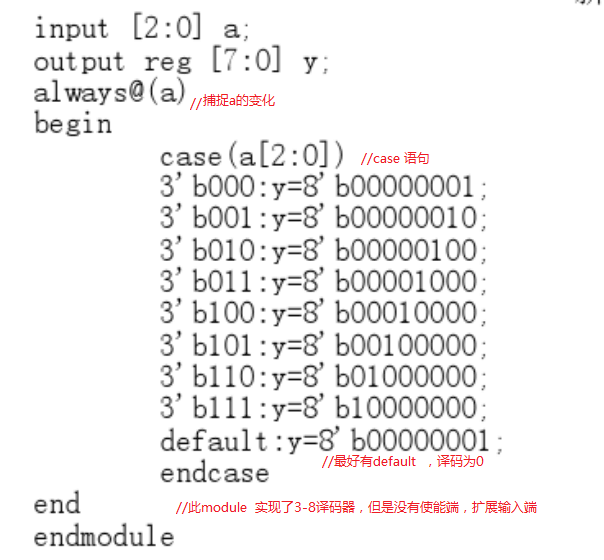
\includegraphics[width=1\textwidth]{lab04_cd.png}
\end{figure}
\subsection{波形图}
\begin{figure}[H]
  \centering
  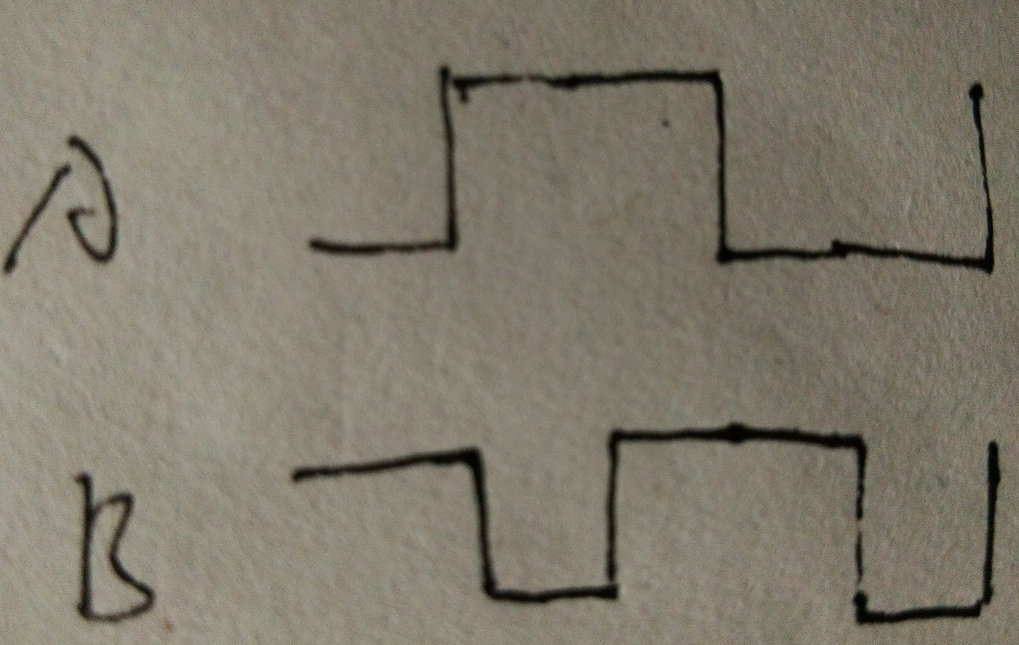
\includegraphics[width=1\textwidth]{wave.png}
\end{figure}


\section{源代码}

\begin{lstlisting}[language=verilog]
module top(
        input rst,clk,
        output [7:0] seg ,[2:0] AN,[3:0] LED
    );
    wire [29:0] pad;
    cnt2  cnt_ins(.out(pad),.clk(clk),.rst(~rst));
    assign AN=3'b000; 
    assign LED[0]=pad[29],
           LED[1]=pad[28],
           LED[2]=pad[27],
           LED[3]=pad[26];
    decoder  dec_ins(.in(pad[29:26]),.out(seg));
    



module cnt2(
    input clk50m,reset, 
    output reg [29:0] out
    );
    always @(posedge clk50m,posedge reset)
        if(reset) out<=8'h3333_3333;
        else out <=out+1;
endmodule




module decoder(
        input [3:0] in,
        output reg  [7:0] out
        );
        always@(*)
            begin 
                case(in)
                0:out<=8'b1100_0000;
                1:out<=8'b1111_1001;
                2:out<=8'b1010_0100;
                3:out<=8'b1011_0000;                    
                4:out<=8'b1001_1001;
                5:out<=8'b1001_0010;
                6:out<=8'b1000_0010;
                7:out<=8'b1101_1000;
                8:out<=8'b1000_0000;
                9:out<=8'b1001_0000;
                10:out<=8'b1000_1000;
                11:out<=8'b1000_0011;
                12:out<=8'b1100_0110;
                13:out<=8'b1010_0001;
                14:out<=8'b1000_0110;
                15:out<=8'b1000_1110;
                endcase
            end
endmodule
\end{lstlisting}

\end{document}